\documentclass[aspectratio=169]{beamer}  % 16:9 aspect ratio

% Use a clean theme as base
\usetheme{default}
\usecolortheme{default}

% Custom colors from HKUST logo
\definecolor{hkustblue}{RGB}{0, 51, 119}    % Navy blue from logo
\definecolor{hkustgold}{RGB}{180, 141, 61}  % Golden brown from logo
\definecolor{lightgray}{RGB}{236, 240, 241}

% Customize the appearance
\setbeamercolor{structure}{fg=hkustblue}
\setbeamercolor{background canvas}{bg=white}
\setbeamercolor{normal text}{fg=hkustblue}
\setbeamercolor{frametitle}{fg=hkustblue,bg=white}
\setbeamercolor{itemize item}{fg=hkustgold}
\setbeamercolor{itemize subitem}{fg=hkustgold}
\setbeamercolor{block title}{fg=white,bg=hkustblue}
\setbeamercolor{block body}{fg=hkustblue,bg=lightgray}
\setbeamercolor{title}{fg=hkustblue}
\setbeamercolor{subtitle}{fg=hkustgold}

% Remove navigation symbols
\setbeamertemplate{navigation symbols}{}

% Customize frame title
\setbeamertemplate{frametitle}{
    \vspace*{0.5cm}
    \insertframetitle
    \vspace*{0.2cm}
    \begin{beamercolorbox}[wd=\paperwidth,ht=0.2pt]{structure}
    \end{beamercolorbox}
}

% Customize itemize bullets
\setbeamertemplate{itemize item}{\small\raise0.5pt\hbox{\textbullet}}
\setbeamertemplate{itemize subitem}{\tiny\raise1.5pt\hbox{\textbullet}}

% Packages
\usepackage{graphicx}
\usepackage{amsmath}
\usepackage{hyperref}
\usepackage{tikz}
\usetikzlibrary{arrows.meta, positioning}

% Title page information
\title{Foundations of Demand Estimation}
\subtitle{Nonparametric Identification}
\author{ZHANG, Jianhao}
\institute{Hong Kong University of Science and Technology}
\date{\today}


\begin{document}

% Title page
\begin{frame}
    \titlepage
\end{frame}

% Table of contents
\begin{frame}{Outline}
    \tableofcontents
\end{frame}

% Add page number in the footline
\setbeamertemplate{footline}{%
  \leavevmode%
  \hfill%
  \begin{beamercolorbox}[wd=2cm,ht=0.8cm,center]{structure}%
    \usebeamerfont{page number}\insertframenumber/\inserttotalframenumber%
  \end{beamercolorbox}%
  \vspace*{0.2cm}%
}

% Section 1
\section{Nonparametric Identification with Market-level Data}
\begin{frame}{Insights from Parametric Models}
How standard parametric models are identified brings out three recurring themes:
    \begin{itemize}
        \item Demand shocks that enter through indices for each good.
        \item The presence of a one-to-one mapping between the indices and market shares, allowing inversion of the demand system.
        \item The application of instrumental variables to identify the components of the inverse demand.
    \end{itemize}
\end{frame}

\begin{frame}{Nonparametric Demand Model}
    Without loss, condition on a fixed number of inside goods \textit{J}, the demand for each product \textit{j} in market \textit{t} can be given by:
    \begin{equation}
        s_{jt} = \sigma_j(x_t, p_t, \xi_t) \qquad j = 1, \ldots, J.
    \end{equation}
    \vspace{-0.5cm}
    \begin{itemize}
        \item \(s_{jt}\), measure of demand at market-level.
        \item \(x_t, all\) observed exogenous characteristics of the market and goods.
        \item \(p_t\), prices of all goods.
        \item \( \xi_{t}\), the \textit{J}-vector of demand shocks.
    \end{itemize}
    To demonstrate identification, Berry and Haile(2014) require three main assumptions.
\end{frame}

\begin{frame}{A Nonparametric Index}
    \begin{block}{\textbf{Assumption 1 (Index)}}
        For all \(j\), \(\sigma_j(x_t, p_t, \xi_t) = \sigma_j\left(x_t^{(2)}, \delta_t, p_t\right)\).
    \end{block}
    \begin{itemize}
        \item Partition \(x_t\) as \((x_t^{(1)}, x_t^{(2)})\) where \(x_t^{(1)} = (x_{1t}^{(1)}, \ldots, x_{Jt}^{(1)}) \in \mathbb{R}^J\).
        \item For each market \(t\), define a vector of indices \(\delta_t = (\delta_{1t}, \ldots, \delta_{Jt})\) where
    \begin{equation}
        \delta_{jt} = x_{jt}^{(1)} \beta_j + \xi_{jt}
    \end{equation}
    \end{itemize}
\end{frame}

\begin{frame}{A Nonparametric Index}
    We may assume without loss of generality that \(E[\xi_{jt}] = 0\) and \(|\beta_j| = 1\) for all \(j\):
    \begin{equation}
        \delta_{jt} = x_{jt}^{(1)} + \xi_{jt}
    \end{equation}
    Furthermore, because variables \(x_t^{(2)}\) is exogenous and play no role in the identification argument, we will henceforth condition on an arbitrary value of \(x_t^{(2)}\) without loss of generality and suppress \(x_t^{(2)}\) in the notation.
\end{frame}

\begin{frame}{Inverting Demand}
    \begin{block}{\textbf{Assumption 2 ((Connected substitutes))}}
    \textbf{(i)} \(\sigma_{k}(\delta_t, p_t)\) is nonincreasing in \(\delta_{jt}\) for all \(j > 0\), \(k \neq j\), and any \((\delta_t, p_t) \in \mathbb{R}^{2J}\); \\
    \textbf{(ii)} For each \((\delta_t, p_t) \in \operatorname{supp}(\delta_t, p_t)\) and any \(\emptyset \neq \mathcal{K} \subseteq \{1, \ldots, J\}\), there exist \(k \in \mathcal{K}\) and \(\ell \notin \mathcal{K}\) such that \(\sigma_{\ell}(\delta_t, p_t)\) is strictly decreasing in \(\delta_{kt}\).
    \end{block}
    Part (i) of Assumption 2 requires that goods be weak substitutes with respect to the indices: an improvement in the index \(\delta_{jt}\) must weakly reduce the demand for other goods.\\
    Part (ii) requires at least some strict substitution among goods \(j = 0, 1, \ldots, J\), that there is no strict subset of goods that substitute only among themselves.
\end{frame}

\begin{frame}{Inverting Demand}
\begin{figure}
        \centering
        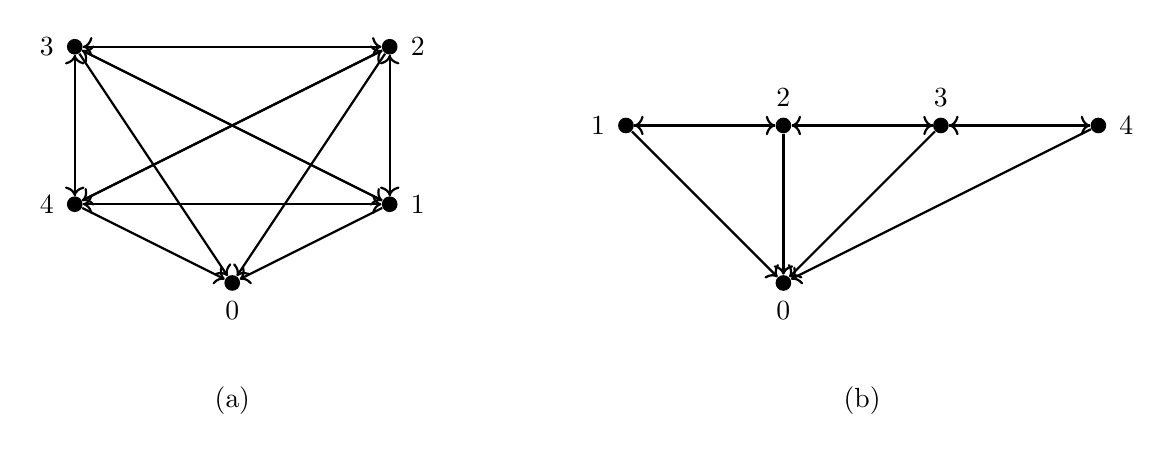
\begin{tikzpicture}[
            node distance=2cm and 2cm,
            every node/.style={circle, fill = black, inner sep = 2pt},
            arrow/.style={->, thick, black}
        ]
        % Left graph (a)
        \node (0) at (0,0) [label=below:0] {};
        \node (1) at (2,1) [label=right:1] {};
        \node (2) at (2,3) [label=right:2] {};
        \node (3) at (-2,3) [label=left:3] {};
        \node (4) at (-2,1) [label=left:4] {};
        
        \draw [arrow] (1) -- (0);
        \draw [arrow] (2) -- (0);
        \draw [arrow] (3) -- (0);
        \draw [arrow] (4) -- (0);
        
        \draw [arrow] (1) -- (2);
        \draw [arrow] (1) -- (3);
        \draw [arrow] (1) -- (4);
        \draw [arrow] (2) -- (3);
        \draw [arrow] (2) -- (4);
        \draw [arrow] (3) -- (4);

        \draw [arrow] (2) -- (1);  
        \draw [arrow] (3) -- (1);  
        \draw [arrow] (4) -- (1);  
        \draw [arrow] (3) -- (2);  
        \draw [arrow] (4) -- (2);  
        \draw [arrow] (4) -- (3); 
        \node at (0, -1.5) [fill=white] {(a)};
        
        % Right graph (b)
        \node (0b) at (7,0) [label=below:0] {};
        \node (1b) at (5,2) [label=left:1] {};
        \node (2b) at (7,2) [label=above:2] {};
        \node (3b) at (9,2) [label=above:3] {};
        \node (4b) at (11,2) [label=right:4] {};
        
        \draw [arrow] (1b) -- (2b);
        \draw [arrow] (2b) -- (3b);
        \draw [arrow] (3b) -- (4b);
        \draw [arrow] (2b) -- (1b);  
        \draw [arrow] (3b) -- (2b);  
        \draw [arrow] (4b) -- (3b);  
        \draw [arrow] (4b) -- (0b);
        \draw [arrow] (3b) -- (0b);
        \draw [arrow] (2b) -- (0b);
        \draw [arrow] (1b) -- (0b);
        
        \node at (8, -1.5) [fill=white] {(b)};
        \end{tikzpicture}
    \end{figure}
\end{frame}

\begin{frame}{Inverting Demand}
    \begin{itemize}
        \item Berry et al. (2013) demonstrate in a wide range of demand models that invertibility of demand is ensured whenever the connected substitutes conditions hold for some injective transformation of the demand system.
        \item Key implication is that for all demand vectors \(s_t\) such that \(s_{jt} > 0\) for all \(j\), there exists an inverse demand system taking the form:
\begin{equation}
    \delta_{jt} = \sigma_j^{-1}(s_t; p_t) \qquad j = 1, \ldots, J.
\end{equation}
    \end{itemize}
\end{frame}

\begin{frame}{Identification via instruments}
    \begin{itemize}
    \item In the case of nonparametric regression we are interested in an equation of the form:
    \begin{equation}
        y = \Gamma(x) + \epsilon
    \end{equation}
    where \(x \in \mathbb{R}^K\). 
    \item  Newey and Powell (2003) showed that given instruments \(z\) satisfying the mean independence condition \(E[\epsilon|z] = 0\), a necessary and sufficient condition for identification of the regression function \(\Gamma\) is a standard "completeness" condition.
    \end{itemize}
\end{frame}

\begin{frame}{Identification via instruments}
    \begin{block}{\textbf{Standard "completeness" condition}(Newey and Powell, 2003)}
        In the class of functions \(B(\cdot)\) on \(\mathbb{R}^K\) such that \(E[B(x)|z]\) is finite, the only function \(B\) such that \(E[B(x)|z] = 0\) almost surely is a function that maps to zero almost surely on its domain. 
    \end{block}
\end{frame}

\begin{frame}{Identification via instruments}
    To connect this to demand, observe that we may re-arrange each equation of (3) as:
    \begin{equation}
        x_{jt}^{(1)} = \sigma_j^{-1}(s_t; p_t) - \xi_{jt}
    \end{equation}
    yielding a form similar to (5).
\end{frame}

\begin{frame}{Identification via instruments}
    \begin{block}{\textbf{Assumption 3 (Instruments)}}
       (i) For all \(j = 1, \ldots, J\), \(E[\xi_{jt} | z_t, x_t^{(1)}] = 0\) almost surely\\
       (ii) For all functions \(B(s_t, p_t)\) with finite expectation, if \(E[B(s_t, p_t) | z_t, x_t^{(1)}] = 0\) almost surely, then \(B(s_t, p_t) = 0\) almost surely.
    \end{block}
    \textbf{Lemma 1.} Under Assumptions 1--3, for all \(j = 1, \ldots, J\), \(\sigma_j^{-1}\) is identified on the support of \((s_t, p_t)\).
\end{frame}

\begin{frame}{Identification via instruments}
    \begin{block}{\textbf{Theorem}(Berry and Haile, 2014).}
       Suppose \((s_t, x_t, p_t, z_t)\) are observable and that Assumptions 1--3 hold. Then for all \(j\), the demand function \(\sigma_j\) is identified.
    \end{block}

\end{frame}

% section 2
\section{Identification with Micro Data}
\begin{frame}{Micro Data}
    \begin{itemize}
        \item "Micro data" refers to a setting where we can observe individual consumer characteristics \(d_{it}\) matched with the choices \(q_{it}\) of each consumer.
        \item Micro data can also provide a panel structure of observed outcomes for many individual consumers within each market.
    \end{itemize}
\end{frame}


\begin{frame}{Micro Data: Estimation}
    \begin{itemize}
        \item One significant advantage of micro data: the potential for within-market variation to lessen (but not eliminate) reliance on instrumental variables.
        \item Suppose we have a mixed logit specification, with conditional indirect utilities of the form
    \begin{equation}
        u_{ijt} = x_{jt}\beta_{it} - \alpha_0 p_{jt} + \xi_{jt} + \epsilon_{ijt},
    \end{equation}
    where
    \begin{equation}
        \beta_{it}^{(k)} = \beta_0^{(k)} + \sum_{\ell=1}^L \beta_d^{(\ell, k)} d_{i\ell t} + \beta_\nu^{(k)} \nu_{it}^{(k)}.
    \end{equation}
    \end{itemize}
    \end{frame}
    

\begin{frame}{Micro Data: Estimation} 
    We can rewrite this as:
    \begin{equation}
        u_{ijt} = \delta_{jt} + \mu_{ijt}(\nu_{it}; \beta_d, \beta_\nu) + \epsilon_{ijt},
    \end{equation}
    with
    \begin{equation}
        \mu_{ijt}(\nu_{it}; \beta_d, \beta_\nu) = \sum_{k=1}^K x_{jt}^{(k)} \left( \beta_\nu^{(k)} \nu_{it}^{(k)} + \sum_{\ell=1}^L \beta_d^{(\ell, k)} d_{i\ell t} \right)
    \end{equation}
    and
    \begin{equation}
        \delta_{jt} = x_{jt} \beta_0 - \alpha_0 p_{jt} + \xi_{jt}.
    \end{equation}
    McFadden et al.(1977) referred to  \(\delta_{jt}\) as the “alternative-specific” constant.
\end{frame}

\begin{frame}{Micro Data: Estimation}  
    \begin{itemize}
    \item With the specification above, choice probabilities for each consumer \(i\) take the form:
    \begin{equation}
        s_{ijt} = \int \frac{\exp\{\delta_{jt} + \mu_{ijt}(\nu_{it}; \beta_d, \beta_\nu)\}}{\sum_{k=0}^{J_t} \exp\{\delta_{kt} + \mu_{ikt}(\nu_{it}; \beta_d, \beta_\nu)\}} dF_{\nu}(\nu_{it})
    \end{equation}
    \item If \(j\) denote the good selected by consumer \(i\) in market \(t\). The (15) gives the likelihood contribution of consumer \(i\)'s choice as a function of parameters \((\delta, \alpha_y, \beta_d, \beta_\nu)\).
    \end{itemize}
\end{frame}

\begin{frame}{Micro Data: Estimation} 
    \begin{itemize}
    \item 
    When the number of observed consumers per good is large in each market. We could estimate \((\delta, \beta_d, \beta_\nu)\) by maximizing the product of these (simulated) likelihoods over all consumers:
    \begin{equation}
        \mathcal{L}(\delta, \beta_d, \beta_\nu)\ = \prod_{i, t} \int \frac{\exp\{\delta_{j(i)t} + \mu_{ij(i)t}(\nu_{it}; \beta_d, \beta_\nu)\}}{\sum_{k=0}^{J_t} \exp\{\delta_{kt} + \mu_{ikt}(\nu_{it}; \beta_d, \beta_\nu)\}} dF_\nu(\nu_{it})
    \end{equation}
    \item We can run a second-step linear IV regression(different from 2SLS) to estimate the parameters \(\alpha_0 \) and \(\beta_0\).
    \item With micro data, we now require only one excluded instrument.
    \end{itemize}
\end{frame}

\begin{frame}{Micro Data: Estimation} 
    \begin{itemize}
    \item It is more preferable to estimate all parameters at once exploiting both with-market and cross-market variation.
    \item Exploiting all variation can often lead to much more precise estimates.
    \item Estimation using simulated likelihood can be computationally demanding if we want sufficient precision
    \end{itemize}
\end{frame}

\begin{frame}{Micro Data: Moment Condition} 
    To estimate all parameters jointly, one could use moment conditions reflecting the score of the likelihood (16) with respect to \((\delta, \beta_d, \beta_\nu\)) together with orthogonality conditions of the form:
    \begin{equation}
        E\left[ \left( \delta_{jt} - x_{jt} \beta_0 - \alpha_0 p_{jt} \right) z_{jt} \right] = 0,
    \end{equation}
    where \(z_{jt}\) represents the exogenous \(x_{jt}\) combined with excluded instruments for \(p_{jt}\).
\end{frame}

\begin{frame}{Micro Data: Moment Condition} 
    \begin{itemize}
    \item Following Berry et al. (2004a) We can combine moments reflecting market shares with “micro moments” characterizing key features of the joint distribution of consumer \(i\)’s characteristics and the characteristics of her choice \(j(i)\). 
    \item Typical micro moments include covariances, or conditional expectations of consumer characteristics given characteristics of the chosen product (or vice versa).
    \item When we have micro data, we will have more limited reliance on orthogonality conditions: aggregate moment condition can be replaced by micro moments that are sufficient to identify (\(\delta\), \(\beta_d\), \(\beta_\nu\)).
   \end{itemize}
\end{frame}

\begin{frame}{Examples of Estimation from Micro Data}
    \begin{itemize}
        \item Demand for hospital(e.g., Capps er al.(2003), Ho(2009)).
        \item Retail outlets(e.g., Burda et al. (2015))
        \item Residential locations (e.g., Bayer et al. (2007), Diamond(2016))
        \item Automobiles (e.g., Goldberg (1995), Petrin (2002)) 
    \end{itemize}
\end{frame}

\begin{frame}{Consumer Panels}
    \begin{itemize}
        \item Typically, consumer panel data refers to observation of each consumer on multiple choice occasions.
        \item One advantage of a consumer panel is that it provide more information about the role of individual characteristics in determing substitution patterns.
    \end{itemize}
\end{frame}

\begin{frame}{Consumer Panels: Estimation}
    \begin{itemize}
    \item
    We can write likelihood contribution for consumer \(i\), as a function of the parameters \((\delta, \beta_d, \beta_\nu)\).
    \begin{equation}
        s_{ijk m} = \int \left( \frac{e^{\delta_{j m 0} + \mu_{i j m 0}(v_{i m}; \beta_d, \beta_\nu)}}{1 + \sum_\ell e^{\delta_{\ell m 0} + \mu_{i \ell m 0}(v_{i m}; \beta_d, \beta_\nu)}} \right) \left( \frac{e^{\delta_{k m 1} + \mu_{i k m 1}(v_{i m}; \beta_d, \beta_\nu)}}{1 + \sum_\ell e^{\delta_{\ell m 1} + \mu_{i \ell m 1}(v_{i m}; \beta_d, \beta_\nu)}} \right) dF_\nu(\nu_{i m}).
    \end{equation}
    \item Another typical approach would start from the types of aggregate moments and micro moments.
    \end{itemize}
\end{frame}

\begin{frame}{Ranked Choice Data}
    \begin{itemize}
        \item Data on each consumer’s rank ordering of products.
        \item The absence of temporal separation can avoid any question about which stochastic components of the model should be viewed as fixed.
        \item Variation in ranked choice data is ideal for assessing the closest substitutes.
        \item Estimation can proceed along the lines suggested previously: likelihood approach (see Train (2009)) and moment method(see Berry et al. (2004a)).
    \end{itemize}
\end{frame}

\section{Nonparametric Identification with Micro Data}
\begin{frame}{Nonparametric Demand Model}
    Following Berry and Haile(2024), consider a nonparametric model of demand characterized by equations
    \begin{equation}
        s_{ijt} = \sigma_j(d_{it}, y_{it}, x_t, p_t, \xi_t) \qquad j = 1, \ldots, J.
    \end{equation}
    Compared to the model considered in the case of market-level data, here we have added observed individual-specific measures \((d_{it}, y_{it})\) as determinants of demand.
\end{frame}

\begin{frame}{Identification Assumptions}
    In addition to the required degree of variation in \(d_{it}\), choice sets and price instruments, the identification results in Berry and Haile (2024) rely on a set of core assumptions on demand.
    The four main assumptions are:
    \begin{itemize}
        \item[(i)] For all \(j\), \(\sigma_j(d_{it}, y_{it}, p_t, \xi_t) = \sigma_j(\gamma(d_{it}, y_{it}, \xi_t), y_{it}, p_t)\), with \(\gamma(d_{it}, y_{it}, \xi_t) \in \mathbb{R}^J\).
        \item[(ii)] \(\sigma(\cdot, y_{it}, p_t)\) is injective on the support of \(\gamma(d_{it}, y_{it}, \xi_t)\) conditional on \((y_{it}, p_t)\).
        \item[(iii)] \(\gamma(\cdot, y_{it}, \xi_t)\) is injective on the support of \(d_{it}|y_{it}\).
        \item[(iv)] For all \(j\), \(\gamma_j(d_{it}, y_{it}, \xi_t) = g_j(d_{it}, y_{it}) + \xi_{jt}\).
    \end{itemize}
\end{frame}

\begin{frame}{Connection to Parametric Model}
    Consider the mixed-logit random utility specification:
    \begin{equation}
        u_{ijt} = x_{jt} \beta_{ijt} - \alpha_{it} p_{jt} + \xi_{jt} + \epsilon_{ijt},
    \end{equation}
    \begin{itemize}
    \item where \(\beta_{ijt}^{(k)} = \beta_{0j}^{(k)} + \sum_{\ell=1}^L \beta_{dj}^{(\ell, k)} d_{i\ell t} + \beta_{\nu j}^{(k)} \nu_{it}^{(k)}\);
    \item \(\ln(\alpha_{it}) = \alpha_0 + \alpha_y y_{it} + \alpha_\nu \nu_{it}^{(0)}\). 
    \end{itemize}
\end{frame}

\begin{frame}{Connection to Parametric Model}
    \begin{itemize}
    \item We can rewrite (20) as 
    \begin{equation}
        u_{ijt} = g_j(d_{it}, x_t) + \xi_{jt} + \mu_{ijt},
    \end{equation}
    where
    \begin{equation}
        g_j(d_{it}, x_t) = \sum_k x_{jt}^{(k)} \sum_{\ell=1}^L \beta_{dj}^{(\ell, k)} d_{i\ell t} = \sum_{\ell=1}^L d_{i\ell t} \sum_k x_{jt}^{(k)} \beta_{dj}^{(\ell, k)}
    \end{equation}
    and
    \begin{equation}
        \mu_{ijt} = \sum_k x_{jt}^{(k)} \left( \beta_{0j}^{(k)} + \beta_{vj}^{(k)} v_{it}^{(k)} \right) - p_{jt} \exp(\alpha_0 + \alpha_y y_{it} + \alpha_\nu \nu_{it}^{(0)}) + \epsilon_{ijt}
    \end{equation}
    \item Notice that if \(L = J\), our key assumptions hold as long as the \(J \times J\) matrix of coefficients on \(d_{it}\) (whose elements are \(\sum_k x_{jt}^{(k)} \beta_{dj}^{(\ell, k)}\)) is full rank.
    \end{itemize}
\end{frame}

 
\begin{frame}{Identification: A Sketch}
    \begin{itemize}
    \item First, a combination of within-market and cross-market variation is exploited to uncover the index function \(g: \mathbb{R}^J \rightarrow \mathbb{R}^J\). 
    \item Then cross-market variation—including that produced by excluded instruments for prices—allows identification of the demand shocks \(\xi_{jt}\) for all goods and markets in the same way that residuals in a nonparametric regression
    model are identified
    \item Finally, with the demand shocks known, identification of demand is immediate from the definition of demand in (19).
    \end{itemize}
\end{frame}
 
 
\begin{frame}{Identification of Index Function}
    \begin{itemize}
    \item Let \(\mathcal{S}(\xi, p)\) denote the support of the share vector when the random variables \((\xi_t, p_t)\) take the values \((\xi, p)\). Because \(d_{it}\) varies within each market, the set \(\mathcal{S}(\xi, p)\) is not a singleton: each \(d_{it}\) in market \(t\) is associated with a different observed conditional choice probability vector \(s_{it}\).
    \item Given the assumptions on demand, for each vector of market shares \(s \in \mathcal{S}(\xi, p)\) there will be a unique \(d^*\) in the support of \(d_{it}\) such that
    \begin{equation}
        \sigma(g(d^*) + \xi, p) = s.
    \end{equation}
    \end{itemize}
\end{frame}

\begin{frame}{Identification of Index Function}
    \begin{itemize}
    \item This \(d^*\) is the vector of consumer characteristics that generate the choice probability vector \(s\) (given \((\xi_t, p_t) = (\xi, p)\)). So we may write
    \begin{equation}
        d^*(s; \xi, p).
    \end{equation}
    \item Furthermore, the inverted demand system at this point is
    \begin{equation}
        g(d^*(s; \xi, p)) + \xi = \sigma^{-1}(s; p).
    \end{equation}
    \item Choice probabilities conditional on \(d_{it}\) in each market \(t\) are observed, \(d^*(s; \xi_t, p_t)\) is observed for all \(t\) and \(s \in \mathcal{S}(\xi_t, p_t)\) even though no \(\xi_t\) is observed or known at this point.
    \end{itemize}
\end{frame}

\begin{frame}{Identification of Index Function}
    \begin{itemize}
    \item If we differentiate (26) within a market \(t\) where \(p_t = p\) and \(d^*(s; \xi_t, p) = d\), we obtain
    \begin{equation}
        \frac{\partial g(d)}{\partial d} \frac{\partial d^*(s; \xi_t, p)}{\partial s} = \frac{\partial \sigma^{-1}(s; p)}{\partial s}.
    \end{equation}
    \item If we do the same within another market \(t'\) with the same \(p\) and same \(s \in \mathcal{S}(\xi_{t'}, p)\), we get a similar expression with an identical right-hand side. Setting the two left-hand sides equal and letting \(d' = d^*(s; \xi_{t'}, p)\), we see that
    \begin{equation}
        \frac{\partial g(d')}{\partial d} = \left[ \frac{\partial g(d)}{\partial d} \right] \frac{\partial d^*(s; \xi_t, p)}{\partial s} \left[ \frac{\partial d^*(s; \xi_{t'}, p)}{\partial s} \right]^{-1}.
    \end{equation}
    \end{itemize}
\end{frame}

\begin{frame}{Identification of Demand}
    \begin{itemize}
    \item Berry and Haile (2024) require that there exist some "common choice probability" vector \(s^*\) that is reached in every market by a consumer with the "right" characteristics \(d_{it}\) for that market. 
    \item Specifically, to our earlier assumptions (i)-(iv) we add:
        \begin{itemize}
        \item[(v)] There exists \(s^*\) such that \(s^* \in \mathcal{S}(\xi, p)\) for all \((\xi, p) \in \text{supp}(\xi_t, p_t)\).
        \end{itemize}
    \item This assumption requires existence of at least one vector of choice probabilities for the inside goods is reached in every market \(t\).
    \end{itemize}
\end{frame}

\begin{frame}{Identification of Demand}
    \begin{itemize}
    \item With a common choice probability vector \(s^*\), in every market \(t\) we have \(J\) inverse demand equations of the form
        \begin{equation}
            g_j(d^*(s^*; \xi_t, p_t)) = \sigma_j^{-1}(s^*; p_t) - \xi_{jt}.
        \end{equation}
    \item Identification of \(\sigma_j^{-1}(s^*; p_t)\) will be done given instruments for endogenous varialbles \(p_t\).
    \end{itemize}
\end{frame}

\begin{frame}
    \thispagestyle{empty}
    \centering
    \Huge
    \textbf{THANK YOU}
\end{frame}

\end{document} 